\begin{figure}[t]
    \centering
    \subfloat[relationship among scenes]{\resizebox{0.22\textwidth}{!}{
        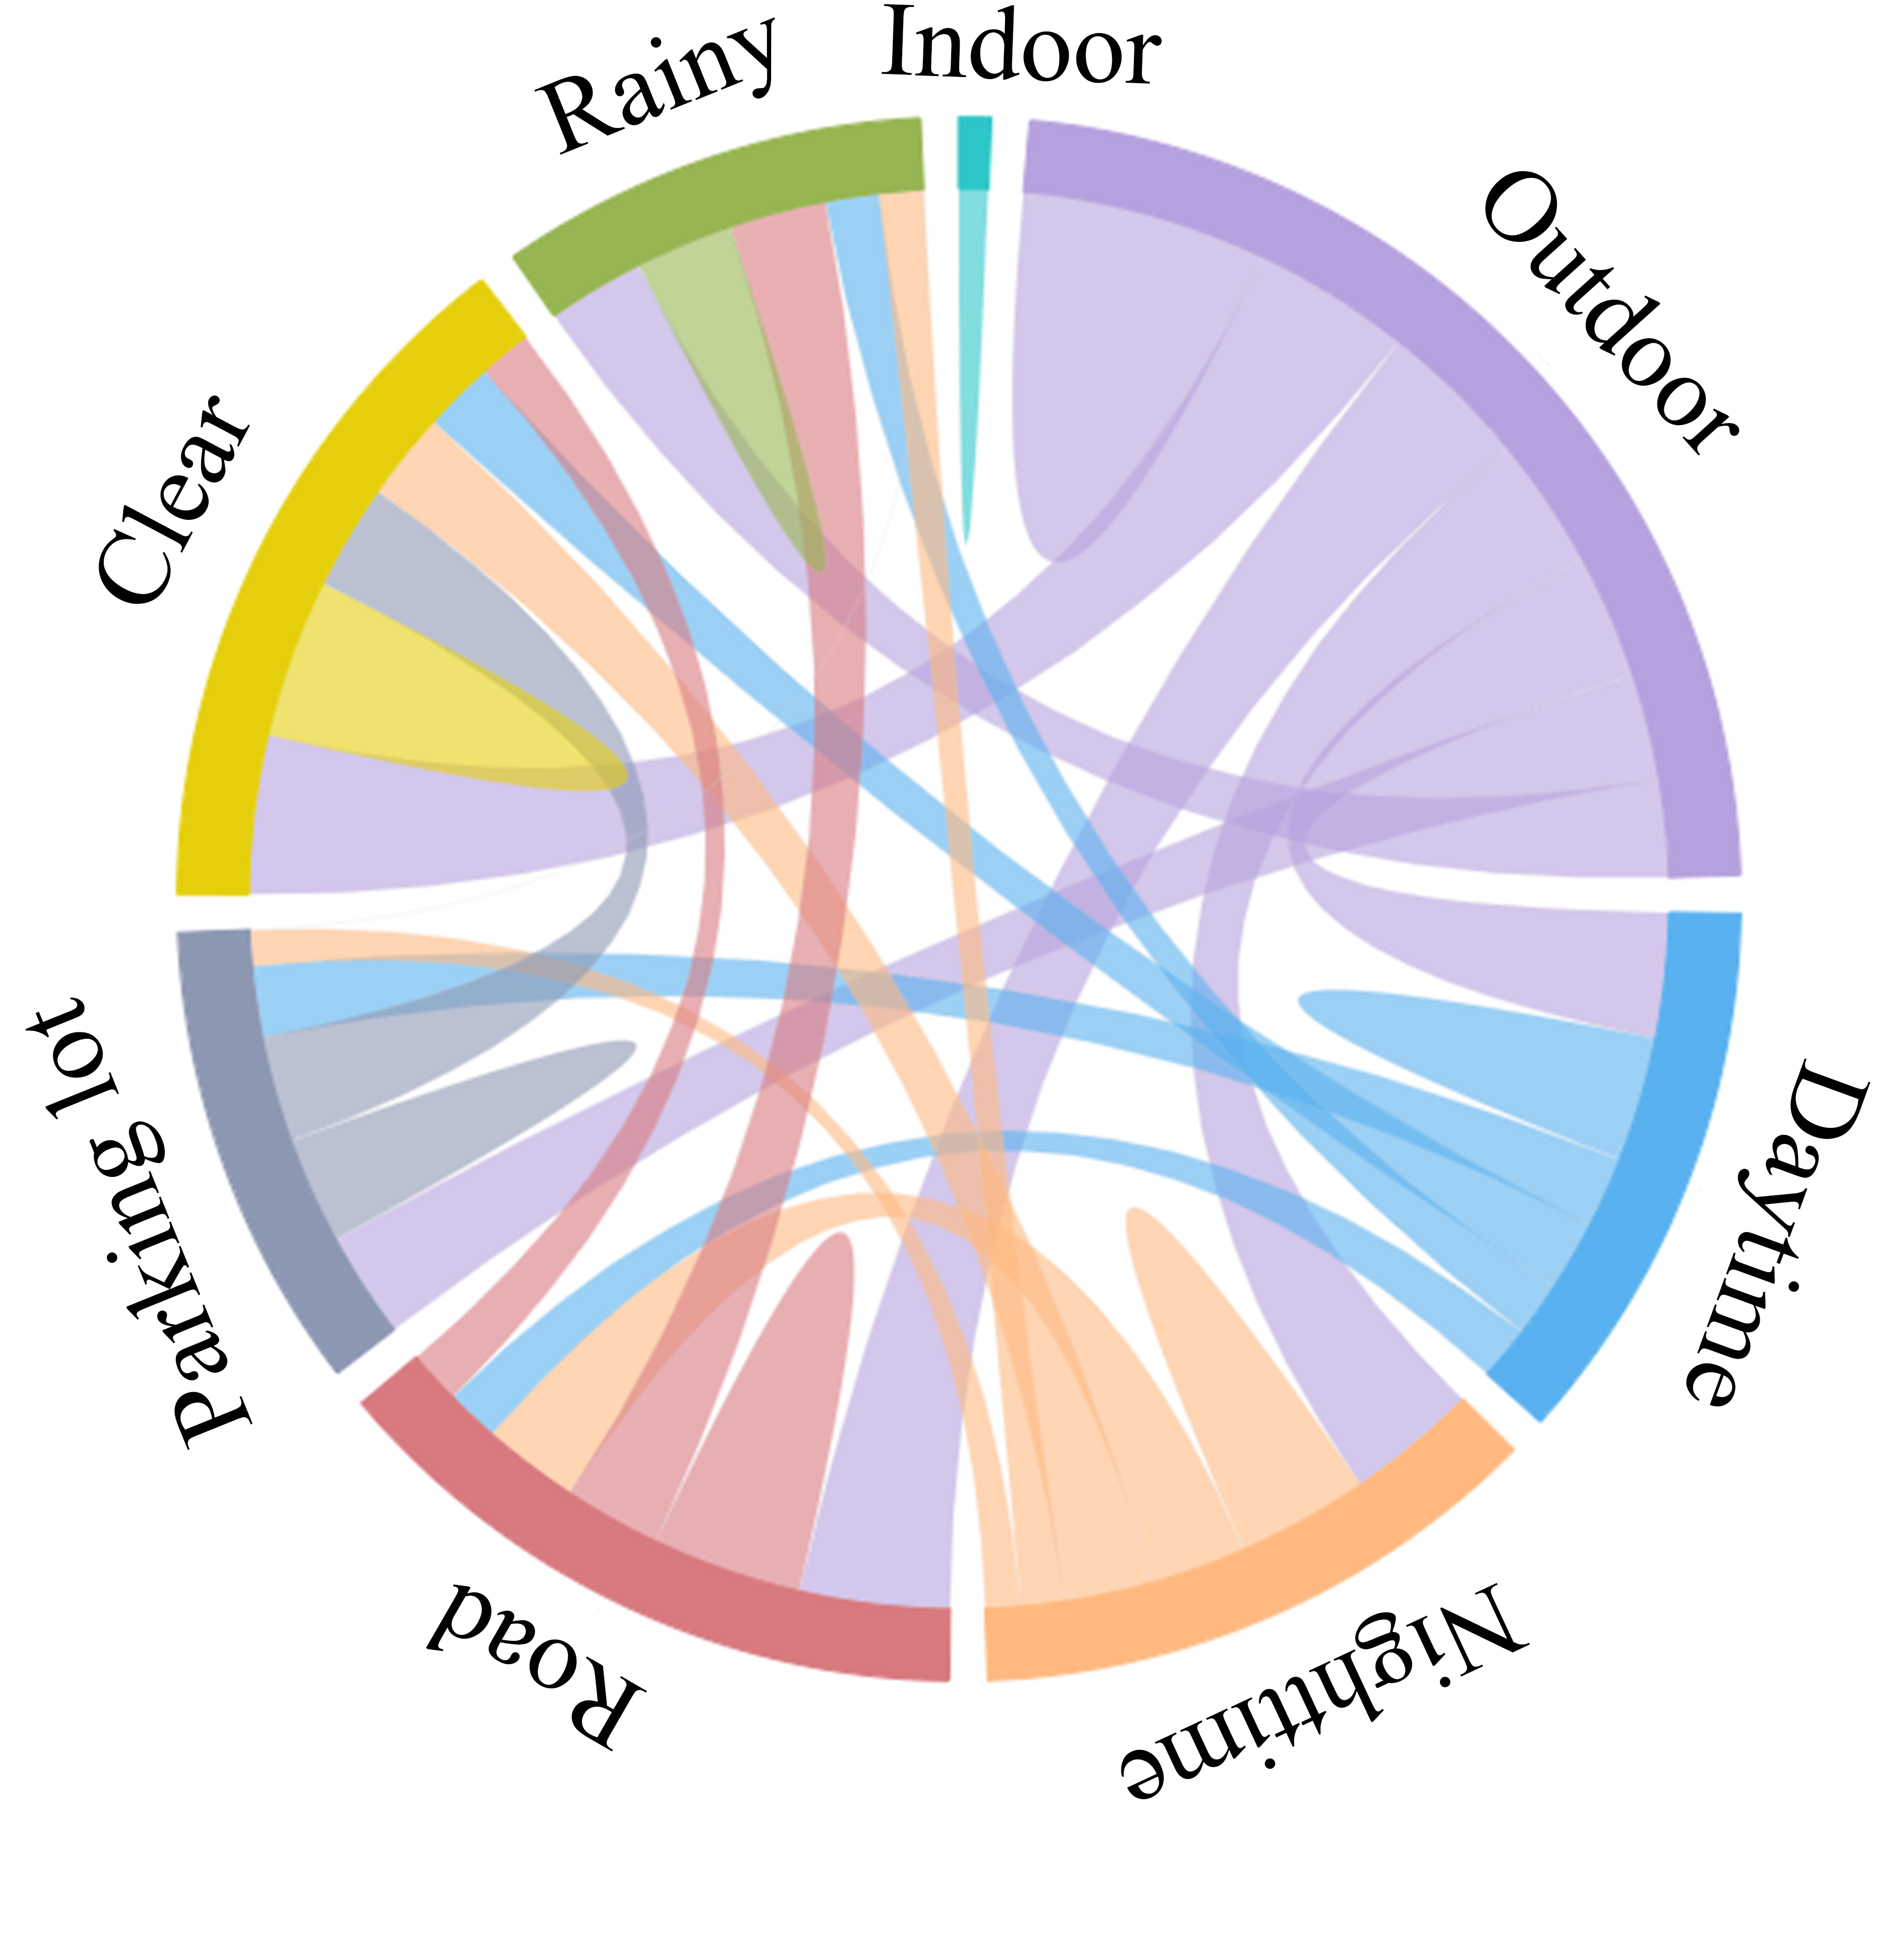
\includegraphics[]{figure/chord.png}
    }}
    \hspace{4mm}
    \subfloat[car instance $ln$ distribution]{\resizebox{0.22\textwidth}{!}{
        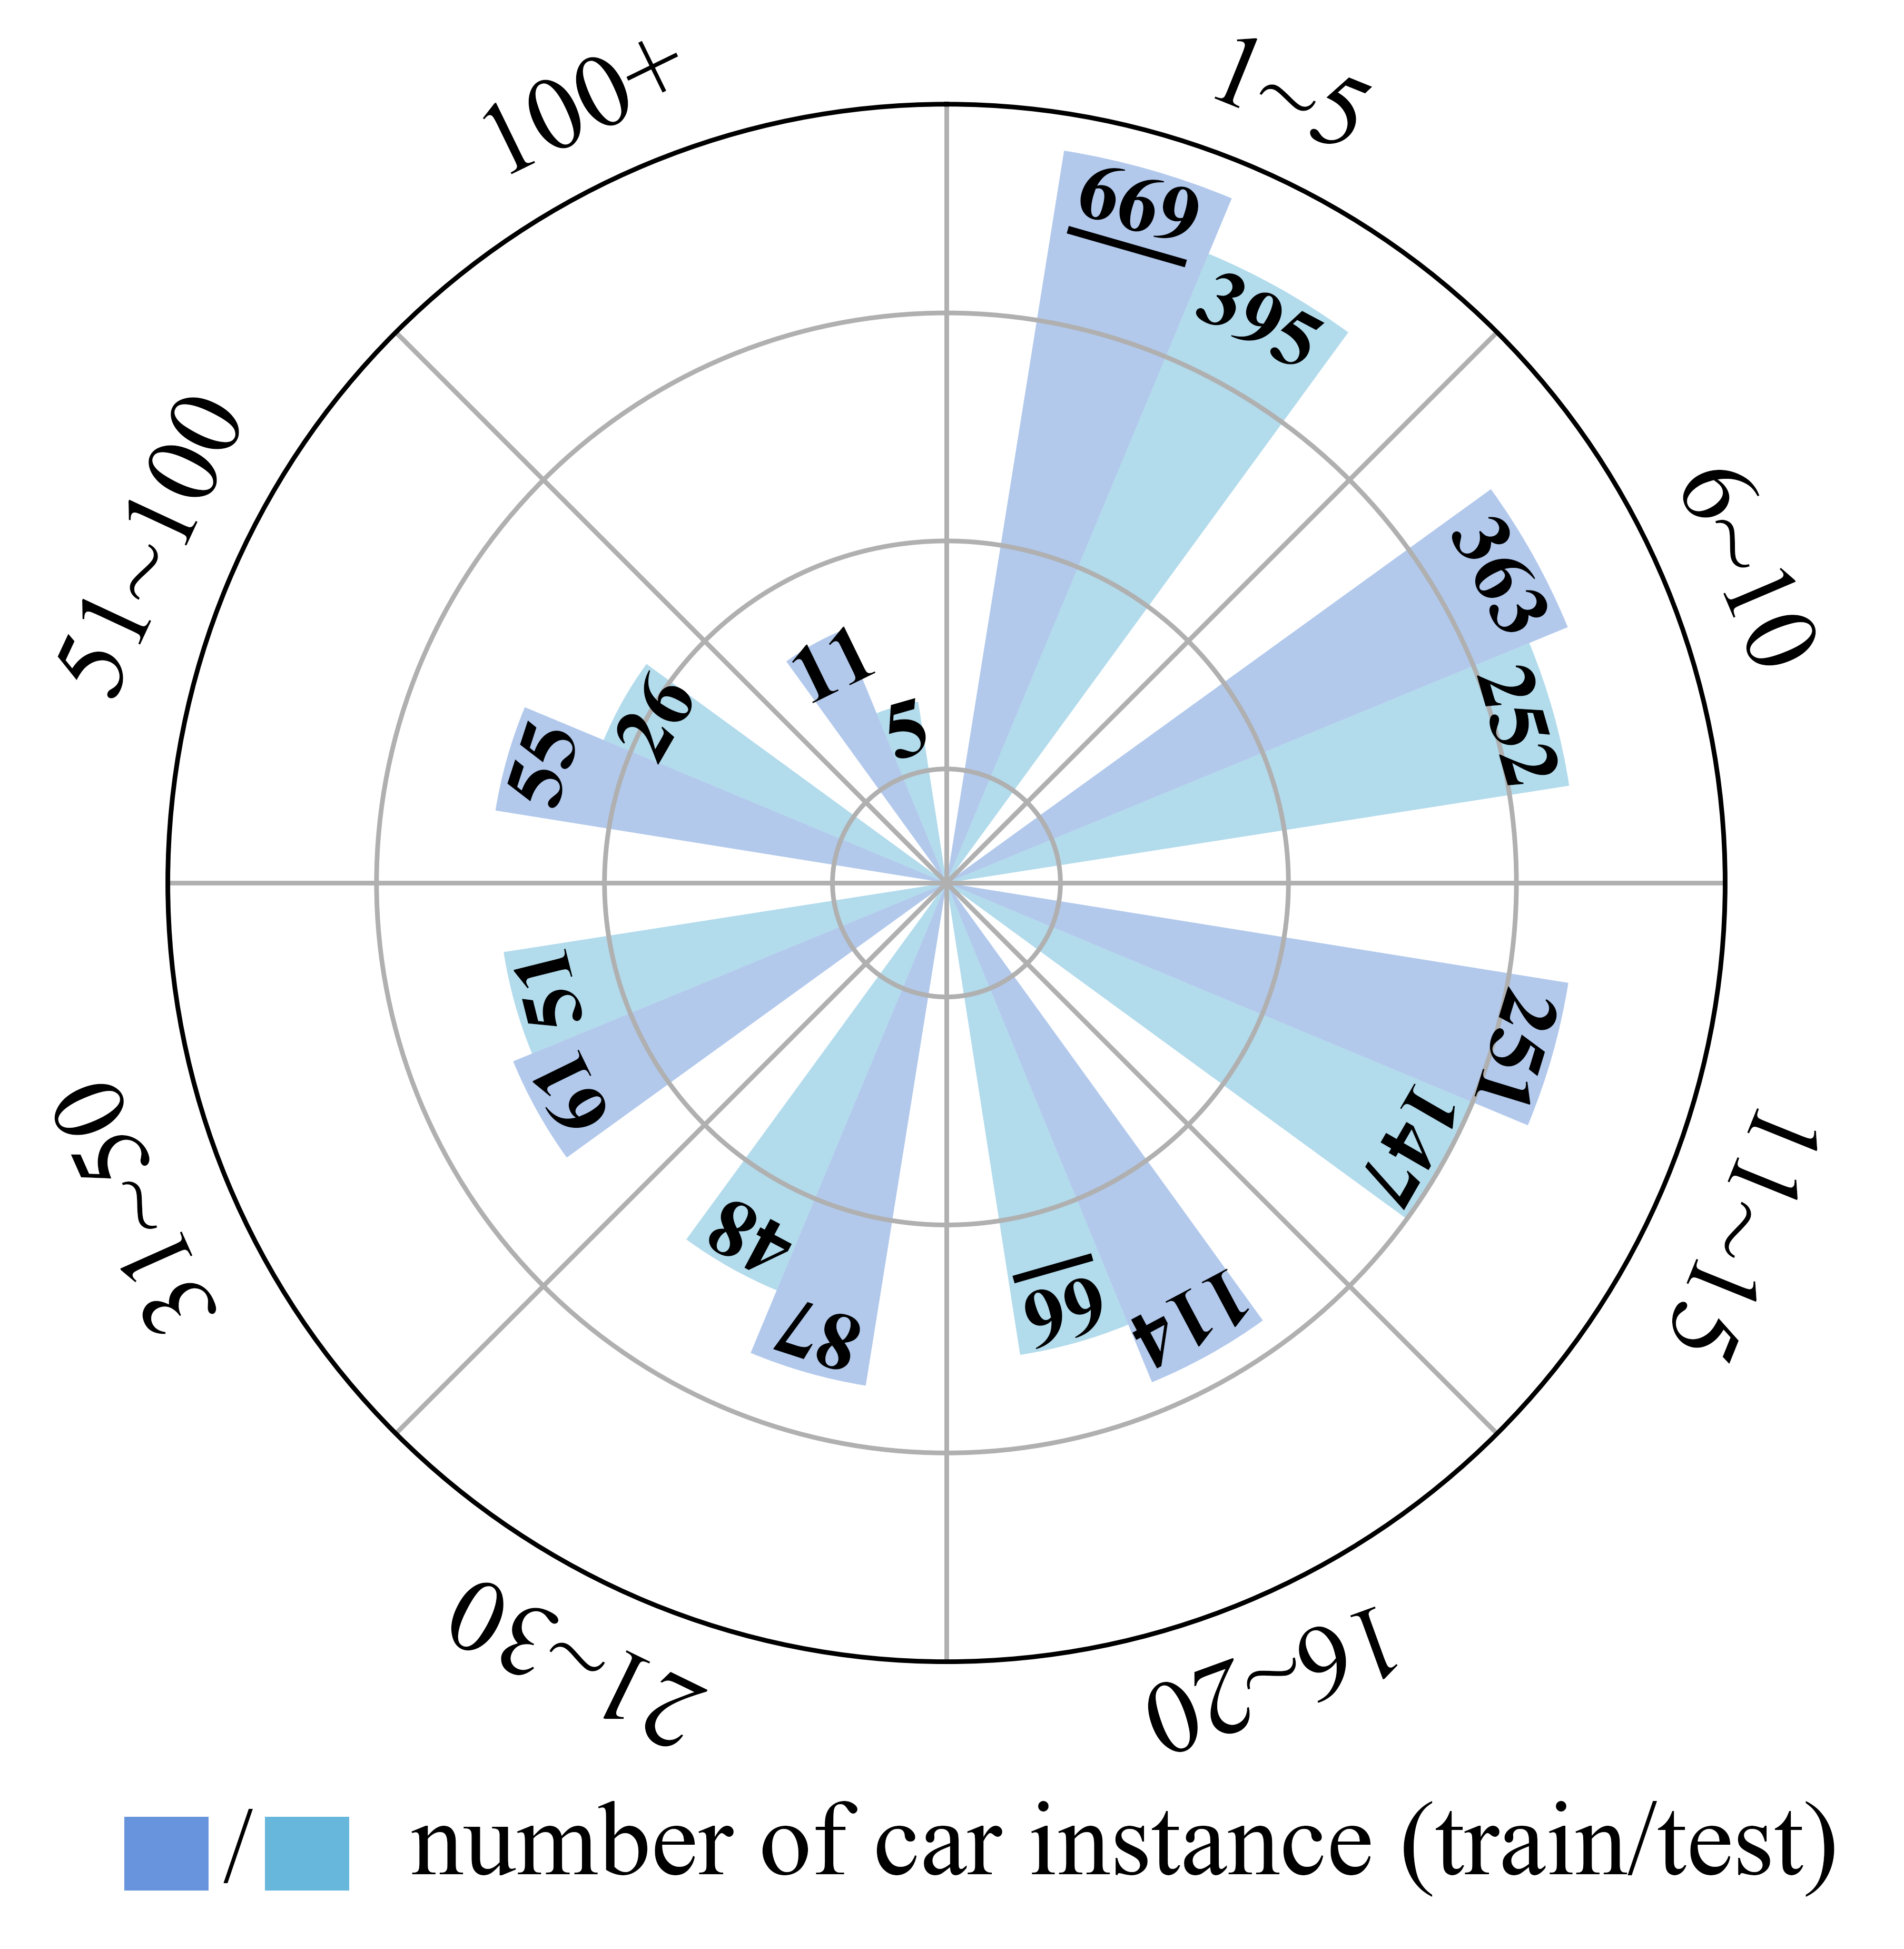
\includegraphics[]{figure/polar.png}
    }}
    \caption{The images in our RGB-P Car dataset vary in terms of (a) scenarios and (b) the number of car instances.}
    \label{fig:dataset}
\end{figure}

\begin{table}[tp]
\caption{Comparison of existing car detection datasets with polarization measurements.}
\small
\centering
\setlength{\tabcolsep}{2.6pt}
\begin{tabular}{c|c|c|c|c}
\hline\hline
Datasets         & Pol. & \begin{tabular}[c]{@{}c@{}}Pixel\\ align\end{tabular} & \begin{tabular}[c]{@{}c@{}}Num.images \\ Train / Test\end{tabular} & \begin{tabular}[c]{@{}c@{}}Num. cars \\ Train / Test \end{tabular} \\ 
\hline
PolarLITIS       & Mono & $\times$                                                     & \begin{tabular}[c]{@{}c@{}}2569 \\ 1640 / 929 \end{tabular}         & \begin{tabular}[c]{@{}c@{}}17428\\ 6061 / 11367 \end{tabular}    \\
\hline
\textbf{RGBP-Car (Ours)} & Tri  & \checkmark                                                     & \begin{tabular}[c]{@{}c@{}}2601 \\ 1611 / 990 \end{tabular}         & \begin{tabular}[c]{@{}c@{}}31234 \\ 19582 / 11652 \end{tabular}   \\ 
\hline\hline
\end{tabular}
\label{tab:datasetcomp}
\end{table}


\section{RGB-P Car Detection Dataset}
\label{sec:dataset}
We construct the first pixel-aligned RGB-polarization car detection dataset called RGBP-Car with trichromatic polarization measurements. We record cars in diverse traffic scenes using FLIR-Blackfly-S, a polarized color camera that simultaneously obtain pixel-aligned polarization measurements in four linear polarization directions (0$^\circ$, 45$^\circ$, 90$^\circ$, and 135$^\circ$) for each color channel (\textit{i.e.}, R, G, and B). RGBP-Car contains 2601 RGB, AoLP, and DoLP image triplets. Each image has manually labeled bounding boxes indicating the position and size of each car. To ensure the diversity and challenge of our dataset, we take the RGB-P images under different weather conditions (clear and rainy), different lighting conditions (daytime and nighttime), different driving environments (indoor, outdoor, road and parking lot), and different car densities. 
Fig. \ref{fig:samples} gives representative examples and Fig. \ref{fig:dataset} analyzes (a) the relationship among different scenes and (b) the density distribution of car instances. Tab. \ref{tab:datasetcomp} further shows the superiority of our RGBP-Car over existing car detection datasets with polarization measurements.

